\documentclass[a4paper,11pt,abstracton,hidelinks]{scrartcl}
\usepackage{dphil}
\addbibresource{refs.bib}
% hide section numbers
\setcounter{secnumdepth}{0}


\title{
Chapter 5. Recent positive selection for insecticide resistance
}


\author{}


\begin{document}
\renewcommand{\abstractname}{Summary}


\maketitle


%%%%%%%%%%%%%%%%%%%%%%%%%%%%%%%%%%%%%%%%%%%%%%%%%%%%%%%%%%%%%%%%%%%%%%%%%%%%%%%
%%%%%%%%%%%%%%%%%%%%%%%%%%%%%%%%%%%%%%%%%%%%%%%%%%%%%%%%%%%%%%%%%%%%%%%%%%%%%%%
%%%%%%%%%%%%%%%%%%%%%%%%%%%%%%%%%%%%%%%%%%%%%%%%%%%%%%%%%%%%%%%%%%%%%%%%%%%%%%%
\begin{abstract}


In this chapter I continue analysing the Ag1000G phase 1 data resource by performing genome-wide scans for signals of recent positive selection.
%
The primary purpose of these selection scans is to identify genes under selection for insecticide resistance.
%
The evolution of insecticide resistance is a major threat to the control of malaria vectors in sub-Saharan Africa, but we still lack a clear picture of which genes are driving this adaptive response.
%
I apply three selection scan methods to each of the mosquito populations in the Ag1000G phase 1 cohort, and develop a systematic approach to identifying and mapping selection signals within these scans.
%
I use this approach to build a catalog of @@N putative selection signals, and validate this by analysing signals overlapping genes that have a functionally-validated role in insecticide resistance.
%
Finally, I describe a web application that provides a means for exploring these selection signals, and illustrate its use by discovering selection signals at a diacylglycerol kinase gene with a potentially novel role in resistance to organophosphate insecticides.


\end{abstract}


\tableofcontents


%%%%%%%%%%%%%%%%%%%%%%%%%%%%%%%%%%%%%%%%%%%%%%%%%%%%%%%%%%%%%%%%%%%%%%%%%%%%%%%
%%%%%%%%%%%%%%%%%%%%%%%%%%%%%%%%%%%%%%%%%%%%%%%%%%%%%%%%%%%%%%%%%%%%%%%%%%%%%%%
%%%%%%%%%%%%%%%%%%%%%%%%%%%%%%%%%%%%%%%%%%%%%%%%%%%%%%%%%%%%%%%%%%%%%%%%%%%%%%%
\section{Introduction}\label{sec:introduction}


% @@TODO citations


As described in Chapter 1, malaria vector control programmes have massively expanded since the turn of the millennium, with a heavy reliance on insecticide-based interventions~\parencite{Cibulskis2016,Bhatt2015,WHO2019WMR}.
%
Human population distributions and patterns of land use have also changed dramatically, including rapid urbanisation~\parencite{Awumbila2017,OECD2020} and the expansion and intensification of agriculture, where insecticides are also used extensively~\parencite{Otsuka2014,BinswangerMkhize2017,Sternberg2018}.
%
Thus, the environment in which natural malaria vector populations seek food and suitable habitats throughout their multi-stage life cycle has radically altered in recent decades, generating new and complex selection pressures.
%
At the heart of this transformation is the massive scale-up of insecticide-treated bednet (ITN) distribution~\parencite{WHO2005WIN,RBM2008GMAP,WHO2017LLIN,Bhatt2015,Okumu2020}.
%
The proportion of the population at risk sleeping under an ITN has increased from less than 2\% to more than 50\% of the population by 2015~\parencite{Cibulskis2016,Bhatt2015}, although coverage varies substantially between countries~\parencite{WHO2019WMR}.
%
All ITNs are treated with a pyrethroid insecticide which serves both to repel mosquitoes and to kill mosquitoes that come into physical contact with the net~\parencite{WHO2020PQVC,Okumu2020}.
%
ITNs target malaria vector species that are highly anthropophilic, in particular \agam\ and \acol.
%
Unsurprisingly, pyrethroid resistance has become widespread in these species and increased in intensity over the time period of ITN scale-up~\parencite{Hemingway2016,Hancock2020}.


Several molecular mechanisms of pyrethroid resistance are known in malaria vectors~\parencite{Hemingway2016}.
%
Yet there remain substantial and surprising gaps in our knowledge of the genetic changes that have occurred in natural \agam\ and \acol\ populations in response to pyrethroid selection pressure.
%
For example, adaptations affecting cytochrome P450 (CYP) enzymes are known to have occurred in some mosquito populations, inducing pyrethroid resistance by increasing the metabolism of insecticide molecules within the mosquito~\parencite{Ranson2016,Hemingway2016}.
%
This form of metabolic resistance is perceived as a significant threat to the efficacy of ITNs~\parencite{Churcher2016,WHO2017PBOLLIN}.
%
There are currently 108 CYP genes annotated in the \agam\ reference genome~\parencite{GiraldoCalderon2015,AgamP4.12}, of which several have been shown to have the potential to metabolise pyrethroids, but it is still not clear which CYP genes are the primary drivers of adaptation to pyrethroids in natural mosquito populations~\parencite{Mohammed2017}.
%
It is also not clear which populations currently carry CYP-mediated pyrethroid resistance adaptations, and whether the same CYP genes are involved across multiple populations or not.
%
Furthermore, other classes of enzyme such as glutathione S-transferases also have the potential to metabolise insecticides, but their role in the evolution of pyrethroid resistance is unclear~\parencite{Adolfi2019}.
%
Additionally, entirely new molecular mechanisms of pyrethroid resistance have recently been discovered~\parencite{Ingham2020}, opening up the possibility of a much larger adaptive landscape than previously appreciated.


Malaria vectors may also encounter a range of other insecticides during their lifetime, either because of malaria vector control interventions or agricultural use.
%
Indoor residual spraying of insecticides (IRS) coverage has not reached the same level as ITNs, but has nevertheless had a measurable impact on malaria transmission~\parencite{Bhatt2015}, with 10.1\% of the population at risk protected by IRS in 2010, although this has fallen back to 4.5\% in 2019~\parencite{WHO2019WMR}.
%
There is even greater spatial heterogeneity in IRS coverage than for ITNs, with IRS generally reserved for use in high transmission regions~\parencite{WHO2019WMR}.
%
Part of the reduction in IRS coverage in recent years can be attributed to the introduction of more expensive insecticides.
%
In 2010, most IRS programmes used pyrethroids, but by 2018 many had switched to use organophosphates because of pyrethroid resistance, although pyrethroids, carbamates and organochlorines all remain in use~\parencite{WHO2019WMR}.
%
All insecticides used in public health either have been or continue to be used in agriculture, and a major open question remains whether agricultural pesticide use is driving selection for insecticide resistance in malaria vectors~\parencite{Georghiou1990,Nkya2013,Philbert2014,Reid2016}.
%
As IRS programmes continue to switch away from pyrethroids to use other insecticides, it is important to understand which resistance adaptations exist in malaria vector populations, either because of prior use in agriculture or because of prior public health use of insecticides with a similar mode of action~\parencite{Fouet2020}.


Given the variety and heterogeneity of these new selection pressures, evolution is likely to be occurring at multiple loci throughout the genomes of malaria vector species, many of which may be unknown.
%
The availability of data from the Ag1000G project on genetic variation in natural malaria vectors provides a unique opportunity to study the full genomic landscape of recent selection, to discover new adaptations to insecticide resistance, and to compare the genomic profile of adaptation between different species and populations.
%
A number of statistical methods have been developed for performing genome-wide selection scans using high quality whole genome variation data from individuals sampled from natural populations~\parencite{Oleksyk2010,Haasl2015,Vatsiou2016,Pavlidis2017,Booker2017}.
%
These methods work in different ways, but all leverage the fact that recent positive selection leaves a characteristic signature at affected loci, which can be detected against a genomic background where the majority of genes have not experienced recent positive selection.
%
For example, H12~\parencite{Garud2015} detects a localised decrease in haplotype diversity,IHS~\parencite{Voight2006} and XPEHH~\parencite{Sabeti2007} detect a localised increase in haplotype sharing, either within or between populations respectively, and PBS~\parencite{Yi2010,Crawford2017} detects a localised increase in genetic differentiation between populations.
%
These methods are not perfect, having varying power to detect different types of selection under different population demographic scenarios~\parencite{Haasl2015,Vatsiou2016,Pavlidis2017,Booker2017}.
%
They may also correctly detect a signal of selection but fail to provide enough precision to narrow down the target of selection to a single gene.
%
Nevertheless, genome-wide selection scans can provide valuable information about genomic regions under selection, within which candidate genes can be identified and prioritised for further study.


In this chapter I use data from Ag1000G phase 1 to explore the genomic landscape of recent positive selection in \agam\ and \acol\ populations from multiple countries.
%
I integrate results from multiple genome-wide selection scans, and compare selection profiles between species and geographical locations.
%
I also describe an online resource where all selection signals can be searched and browsed, and investigate the strongest selection signals to identify candidate genes driving novel forms of insecticide resistance.
%
The analyses described in this chapter were performed in the context of a broader collaboration with the Ag1000G Analysis Working group, and particularly with my colleague Nick Harding from the MalariaGEN Resource Centre team.
%
Here I focus on those analyses that I devised and performed, but include some results from analyses performed jointly for additional context, and indicate joint contributions within the relevant sections.
%


%%%%%%%%%%%%%%%%%%%%%%%%%%%%%%%%%%%%%%%%%%%%%%%%%%%%%%%%%%%%%%%%%%%%%%%%%%%%%%%
%%%%%%%%%%%%%%%%%%%%%%%%%%%%%%%%%%%%%%%%%%%%%%%%%%%%%%%%%%%%%%%%%%%%%%%%%%%%%%%
%%%%%%%%%%%%%%%%%%%%%%%%%%%%%%%%%%%%%%%%%%%%%%%%%%%%%%%%%%%%%%%%%%%%%%%%%%%%%%%
\section{Results}\label{sec:results}


%%%%%%%%%%%%%%%%%%%%%%%%%%%%%%%%%%%%%%%%%%%%%%%%%%%%%%%%%%%%%%%%%%%%%%%%%%%%%%%
%%%%%%%%%%%%%%%%%%%%%%%%%%%%%%%%%%%%%%%%%%%%%%%%%%%%%%%%%%%%%%%%%%%%%%%%%%%%%%%
\subsection{Genome-wide selection scans}\label{subsec:results-gwss}


Genome-wide selection scans were performed using nucleotide variation data from Ag1000G phase 1, which comprises genotypes in 765 individuals at 41,476,870 biallelic SNPs, phased into haplotypes as described in Chapter 3.
%
Three selection scan methods were chosen because of their power to detect recent positive selection: H12~\parencite{Garud2015}, IHS~\parencite{Voight2006} and XPEHH~\parencite{Sabeti2007}.
%
The Ag1000G phase 1 resource includes data on nine mosquito populations, with two \acol\ populations, five \agam\ populations, and two further populations of uncertain species status, described in Chapter 4.
%
However, the Kenyan population exhibited extremely low levels of genetic diversity across the whole genome when compared with other populations, and in exploratory analyses it was evident that this low diversity was associated with increased noise in genome-wide selection scans.
%
The Kenyan population was therefore excluded from further selection analyses.
%
Population structure analyses also revealed evidence for structure among the Cameroon \agam\ mosquitoes, associated with the different collection sites.
%
Only the Cameroon mosquitoes from the savannah collection sites were therefore included.
%
Thus, eight populations were analysed, with sample size ranging from N=31 (Guinea \agam) to N=103 (Uganda \agam).


H12 and IHS genome-wide selection scans were computed for each population, and XPEHH scans were computed for selected pairs of populations.
%
The XPEHH method is designed to identify genome locations where selection is acting in some populations but not others, and therefore combinations of populations were chosen for these scans to allow for comparisons between species and between geographically distant locations.
%
All together, this comprised a total of 40 genome-wide selection scans.
%
To facilitate the rapid computation of these selection scans on the relatively large Ag1000G data resource, I reimplemented the H12, IHS and XPEHH methods in the scikit-allel software package\footnote{https://github.com/cggh/scikit-allel}, making use of general purpose high-performance scientific computing libraries for the Python programming language.
%
I calibrated and ran the H12 scans, and the IHS and XPEHH scans were run by Nick Harding.
%
Each of these scans produced a test statistic for each segregating SNP or for each of a set of genomic windows, where higher absolute values of the statistic indicate stronger evidence for recent positive selection.


%%%%%%%%%%%%%%%%%%%%%%%%%%%%%%%%%%%%%%%%%%%%%%%%%%%%%%%%%%%%%%%%%%%%%%%%%%%%%%%
%%%%%%%%%%%%%%%%%%%%%%%%%%%%%%%%%%%%%%%%%%%%%%%%%%%%%%%%%%%%%%%%%%%%%%%%%%%%%%%
\subsection{Selection signals at known insecticide resistance loci}\label{subsec:known-loci}


\begin{figure}[t!]
\centering
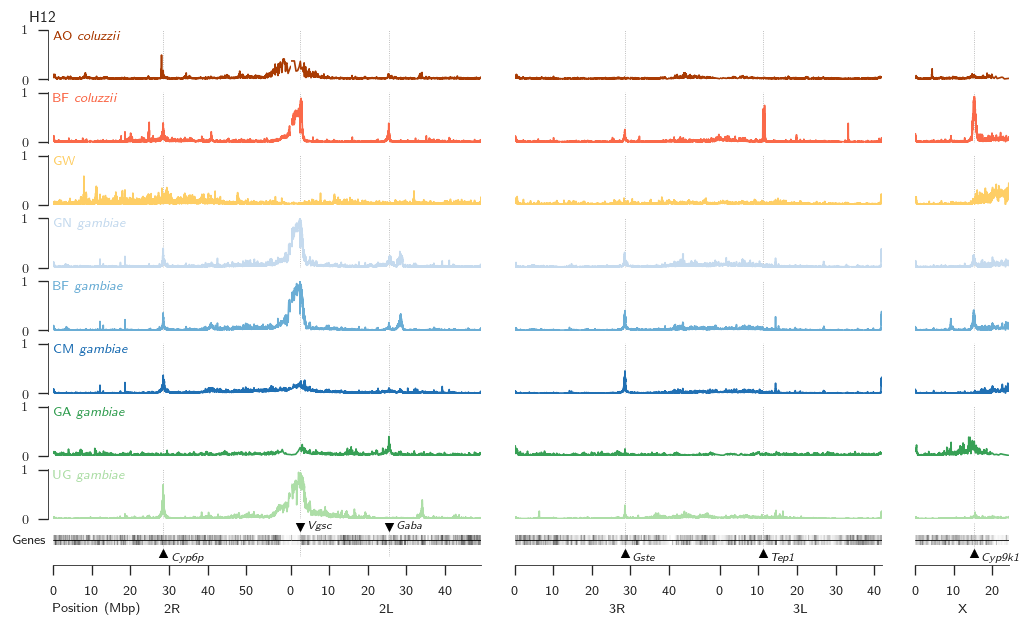
\includegraphics[width=1.1\textwidth,center]{artwork/chapter5/h12.png}
\caption{H12 selection scans.
%
Each track shows results from H12 selection scan in a single population.
%
AO = Angola; BF = Burkina Faso; GW = Guinea-Bissau; GN = Guinea; CM = Cameroon; GA = Gabon; UG = Uganda.
%
H12 values range between 0 and 1, where a value of zero indicates high haplotype diversity within a genomic window, and a value of one indicates low haplotype diversity (at most two distinct haplotypes observed within the sampled individuals).
%
Validated insecticide resistance genes (\textit{Vgsc}, \textit{Gaba}, \textit{Cyp9k1}) or gene clusters (\textit{Cyp6p}, \textit{Gste}) are labelled at the bottom.
%
\textit{Tep1} is an immune system gene previously found to be under selection in \acol~\parencite{White2011}.
% @@TODO stretch this figure!
}
\label{fig:h12}
\end{figure}


To provide an initial view of these data, I plotted the results of the H12 scans over the genome (Fig.~\ref{fig:h12}).
%
There were a number of clear peaks within these scans that were replicated across multiple populations, including at the following five loci containing genes that have been functionally validated as playing a role in insecticide resistance in \agam\ and/or \acol:
%
\begin{itemize}
%%
\item \textbf{2L:2.4 Mb} - This locus contains the voltage-gated sodium channel gene (\textit{Vgsc}; \texttt{AGAP004707}) which encodes a nervous system protein that is the binding target of DDT and pyrethroid insecticides~\parencite{Dong2014}.
%
Amino acid substitutions in this gene confer resistance to DDT and pyrethroids in \agam~\parencite{MartinezTorres1998,Ranson2000a,Jones2012,Wang2015}.
%%
\item \textbf{3R:28.6 Mb} - This locus contains a cluster of eight glutathione S-transferase genes, which encode enzymes involved in detoxification of xenobiotic substances.
%
In \agam\ this locus was initially discovered as a major locus of DDT resistance~\parencite{Prapanthadara1993,Ranson2000b,Ranson2001,Ding2003}.
%
An amino acid substitution in one of the genes in this cluster, \textit{Gste2} (\texttt{AGAP009194}) was subsequently shown to confer elevated DDT resistance~\parencite{Mitchell2014}.
%
Increased expression of \textit{Gste2} has also been shown experimentally to confer resistance to DDT and organophosphates~\parencite{Adolfi2019}.
%%
\item \textbf{2R:28.5 Mb} - This locus contains a cluster of ten genes, nine of which encode cytochrome P450 enzymes.
%
This includes \textit{Cyp6p3} (\texttt{AGAP002865}) which is associated with pyrethroid resistance in \agam\ and is capable of metabolising multiple pyrethroid insecticides~\parencite{Muller2008}.
%
Increased expression of \textit{Cyp6p3} has also been shown experimentally to confer resistance to both pyrethroids and carbamates in \agam~\parencite{Adolfi2019}.
%%
\item \textbf{X:15.2 Mb} - This locus contains the cytochrome P450 gene \textit{Cyp9k1} (\texttt{AGAP000818}).
%
A selection signal has previously been found at this locus in \acol\ in Mali~\parencite{Main2015}.
%
Evolution of \textit{Cyp9k1} has also been observed in \acol\ on Bioko Island in response to combined use of pyrethroids in IRS and ITN programmes~\parencite{Vontas2018}.
%
\textit{Cyp9k1} metabolises the pyrethroid deltamethrin, but also pyriproxyfen, a non-pyrethroid insecticide~\parencite{Vontas2018}.
%%
\item \textbf{2L:25.4 Mb} - This locus contains the \textit{Gaba} gene (\texttt{AGAP006028}) and is also known as the resistance to dieldrin (\textit{Rdl}) locus.
%
This gene encodes another component of the nervous system,  the gamma-aminobutyric acid receptor subunit, which is the binding target for the insecticide dieldrin.
%
Dieldrin use ceased in the 1970s, but resistance has remained persistent in \textit{Anopheles} for decades afterwards~\parencite{Du2005}.
%
Amino acid substitutions are known in \agam\ and \acol\ to confer dieldrin resistance~\parencite{Du2005,Lawniczak2010}.
\end{itemize}


Although these five loci have a known role in insecticide resistance, the fact that there are strong signals of selection in multiple populations in the Ag1000g phase 1 cohort provides valuable confirmation that these loci are indeed playing an important role in adaptation to insecticide pressure in natural malaria vector populations.
%
Because we have a strong prior expectation for selection at these loci, they also provide us with valuable positive controls, allowing us to study the character of true selection signals in more detail.
%
This in turn can guide the design and calibration of algorithms for discovering signals of selection for insecticide resistance at novel loci.


%%%%%%%%%%%%%%%%%%%%%%%%%%%%%%%%%%%%%%%%%%%%%%%%%%%%%%%%%%%%%%%%%%%%%%%%%%%%%%%
%%%%%%%%%%%%%%%%%%%%%%%%%%%%%%%%%%%%%%%%%%%%%%%%%%%%%%%%%%%%%%%%%%%%%%%%%%%%%%%
\subsection{Selection signal discovery and mapping}\label{subsec:signal-discovery}


\begin{figure}[t!]
    \centering
    \begin{subfigure}[t]{0.32\textwidth}
        \centering
        \caption{}
        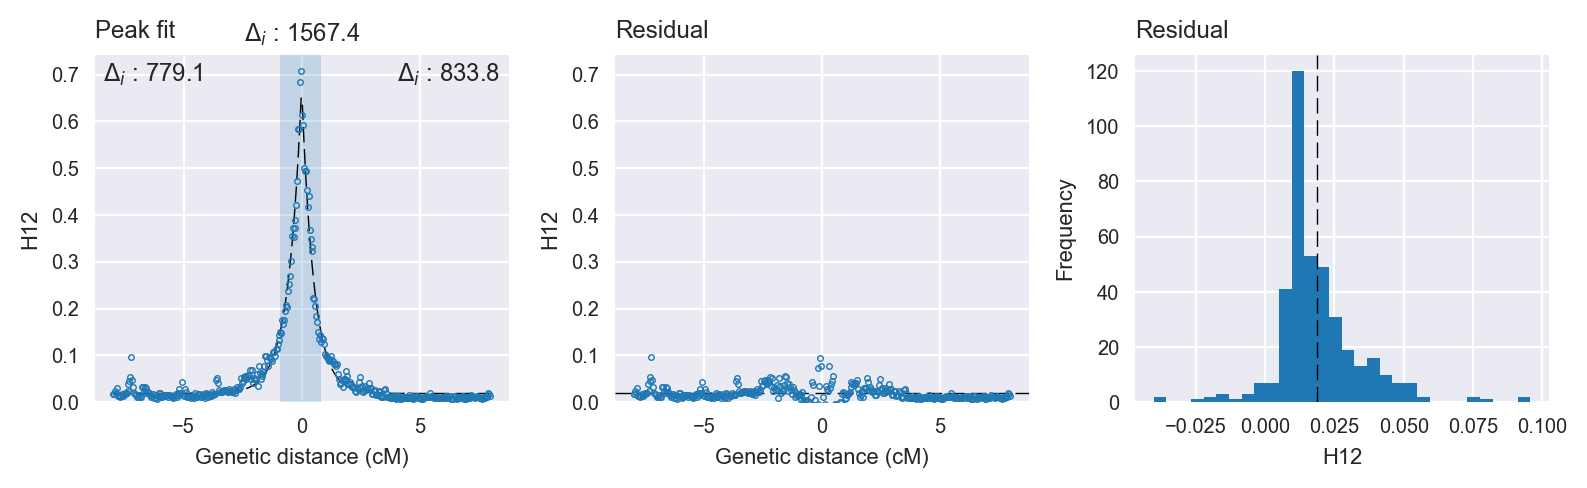
\includegraphics[width=1.1\textwidth,center,trim=0 27 380 0, clip]{artwork/chapter5/peak_fit_h12_cyp6p_ugs.png}
    \end{subfigure}
    \hfill
    \begin{subfigure}[t]{0.32\textwidth}
        \centering
        \caption{}
        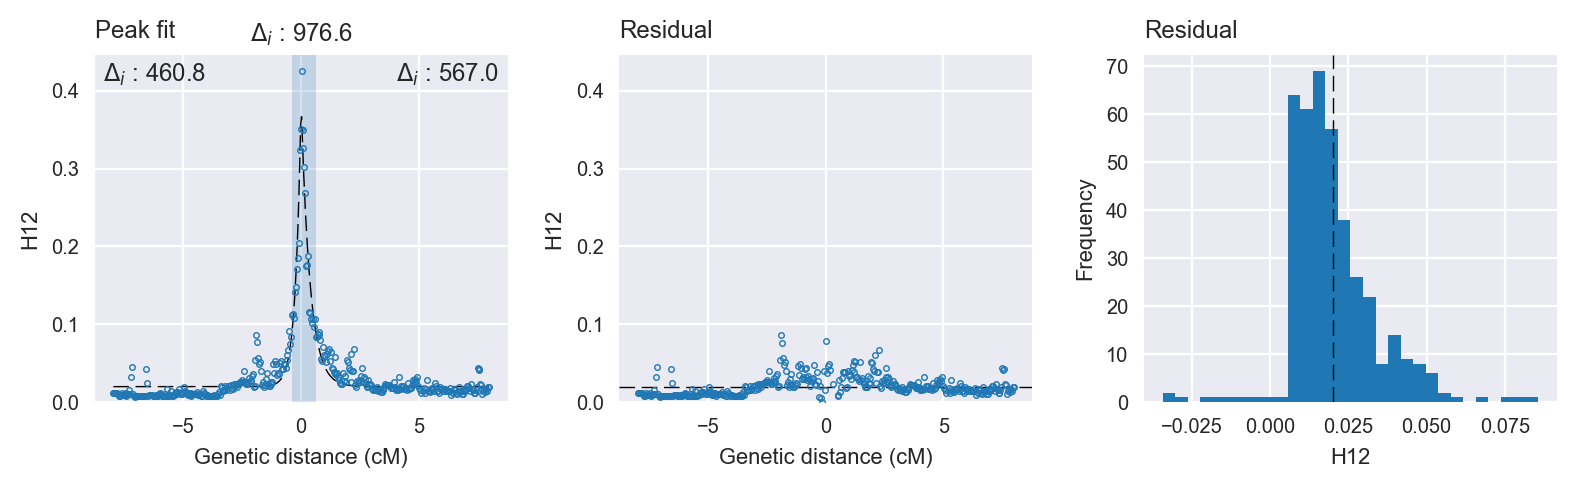
\includegraphics[width=1.1\textwidth,center,trim=0 27 380 0, clip]{artwork/chapter5/peak_fit_h12_cyp6p_bfs.png}
    \end{subfigure}
    \hfill
    \begin{subfigure}[t]{0.32\textwidth}
        \centering
        \caption{}
        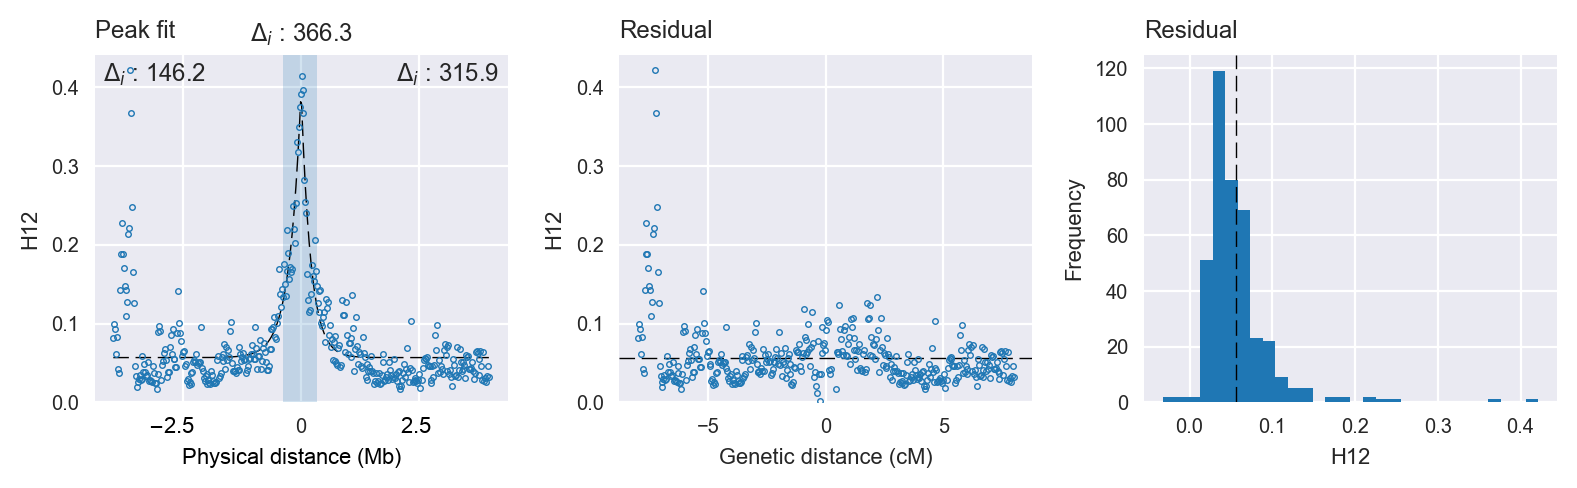
\includegraphics[width=1.1\textwidth,center,trim=0 27 380 0, clip]{artwork/chapter5/peak_fit_h12_cyp6p_bfm.png}
    \end{subfigure}
    \vspace{0cm}
    \begin{subfigure}[t]{0.32\textwidth}
        \centering
        \caption{}
        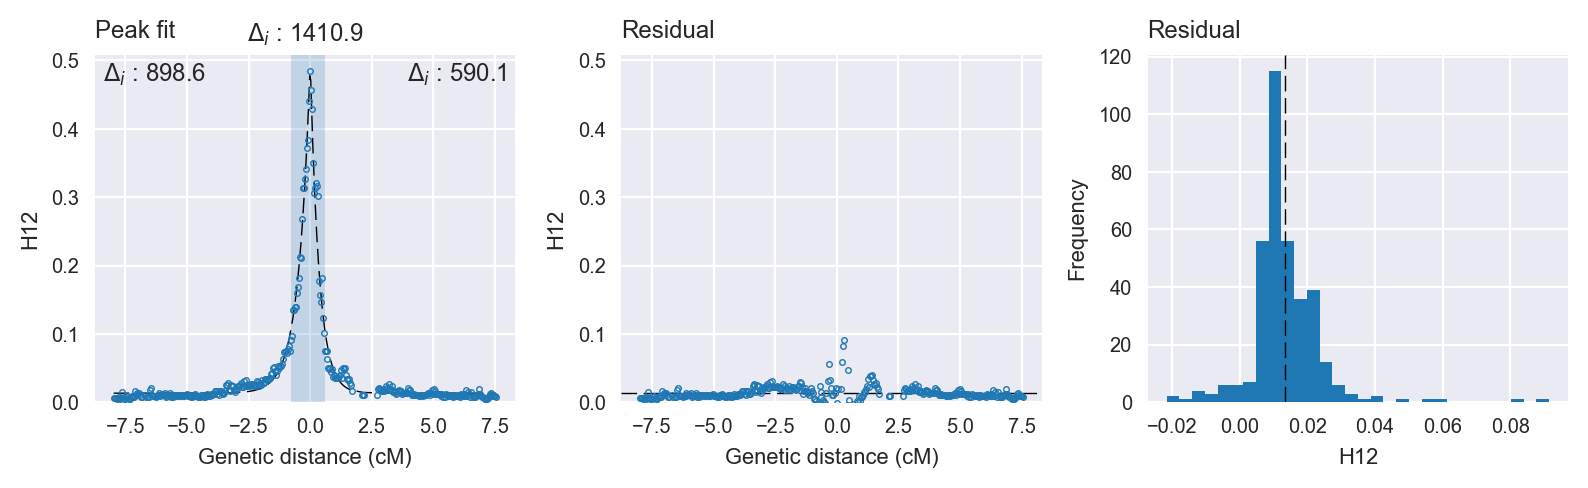
\includegraphics[width=1.1\textwidth,center,trim=0 27 380 0, clip]{artwork/chapter5/peak_fit_h12_gste_cms.png}
    \end{subfigure}
    \hfill
    \begin{subfigure}[t]{0.32\textwidth}
        \centering
        \caption{}
        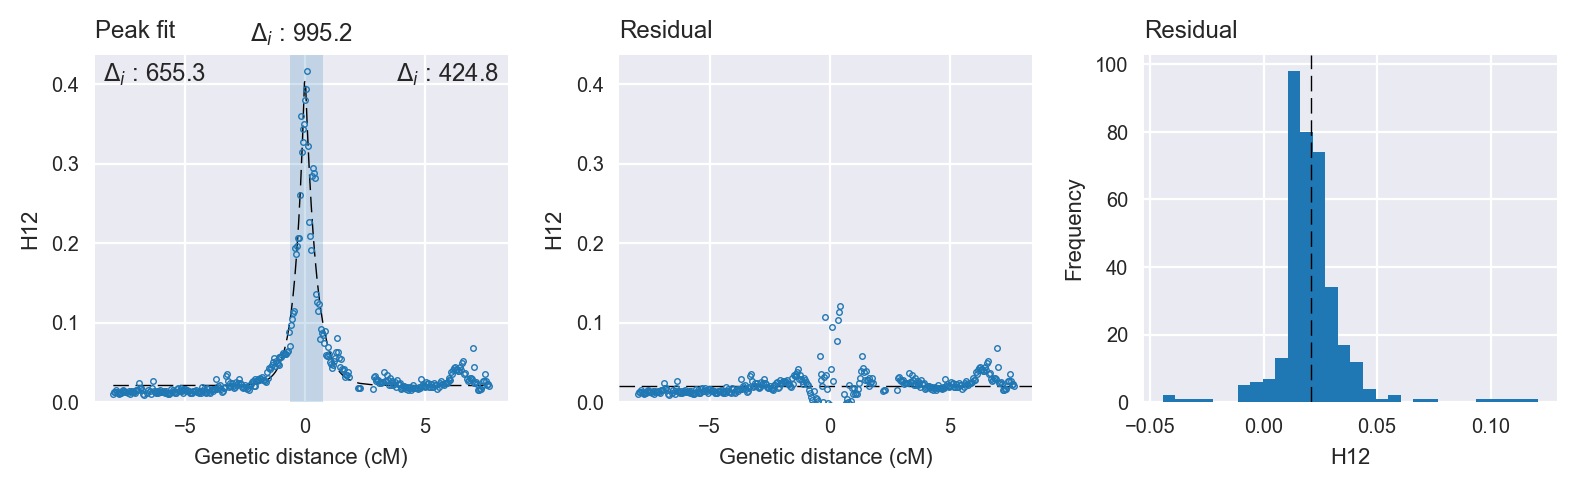
\includegraphics[width=1.1\textwidth,center,trim=0 27 380 0, clip]{artwork/chapter5/peak_fit_h12_gste_bfs.png}
    \end{subfigure}
    \begin{subfigure}[t]{0.32\textwidth}
        \centering
        \caption{}
        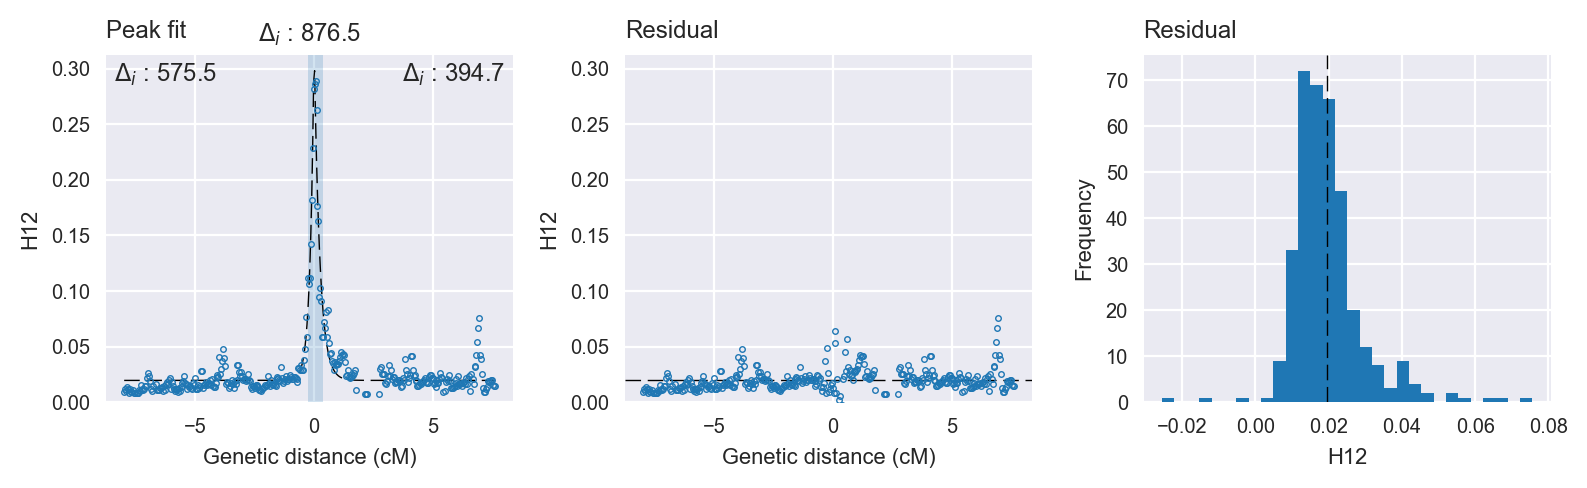
\includegraphics[width=1.1\textwidth,center,trim=0 27 380 0, clip]{artwork/chapter5/peak_fit_h12_gste_ugs.png}
    \end{subfigure}
    \vspace{0cm}
    \begin{subfigure}[t]{0.32\textwidth}
        \centering
        \caption{}
        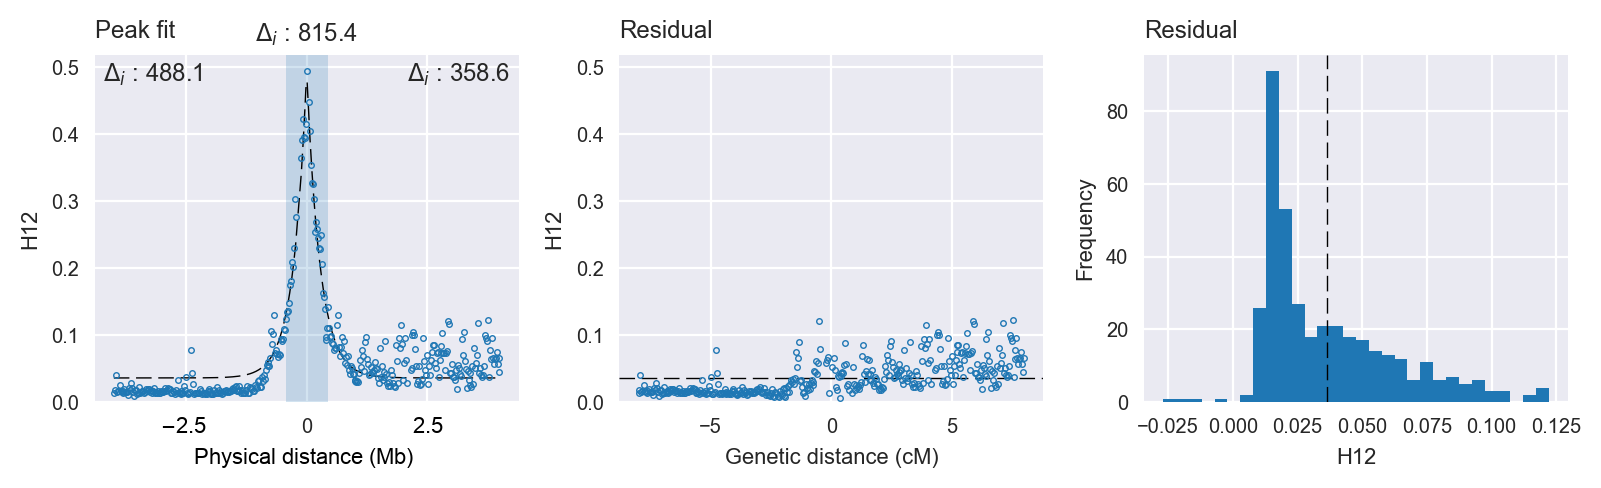
\includegraphics[width=1.1\textwidth,center,trim=0 27 380 0, clip]{artwork/chapter5/peak_fit_h12_cyp9k1_bfs.png}
    \end{subfigure}
    \hfill
    \begin{subfigure}[t]{0.32\textwidth}
        \centering
        \caption{}
        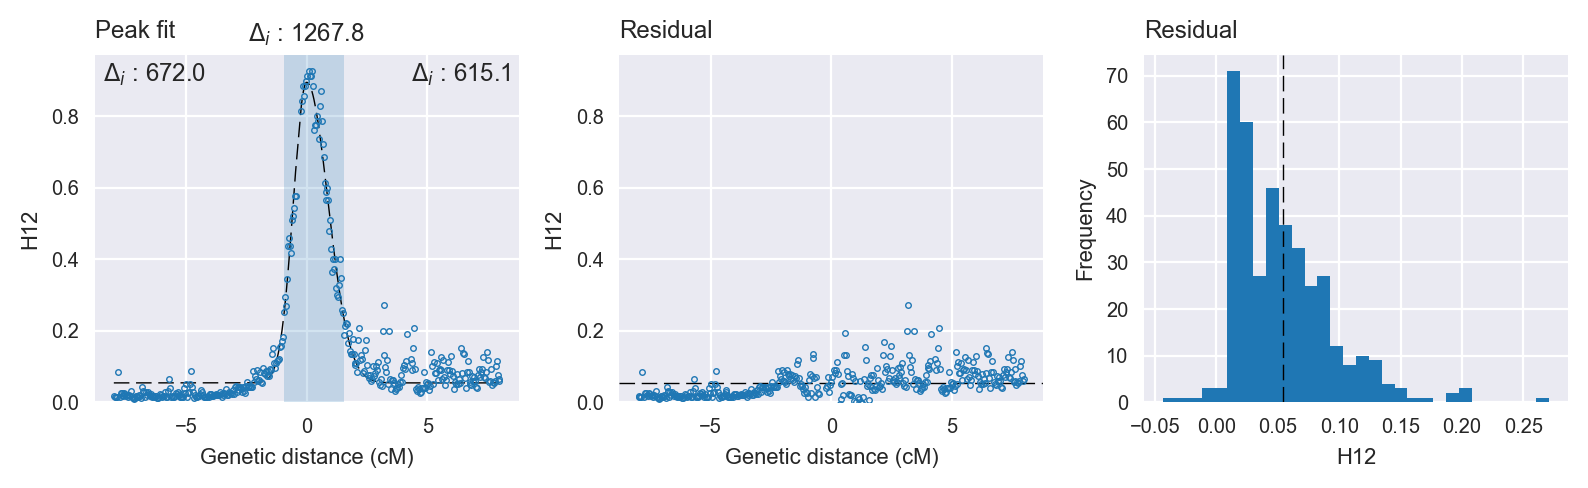
\includegraphics[width=1.1\textwidth,center,trim=0 27 380 0, clip]{artwork/chapter5/peak_fit_h12_cyp9k1_bfm.png}
    \end{subfigure}
    \begin{subfigure}[t]{0.32\textwidth}
        \centering
        \caption{}
        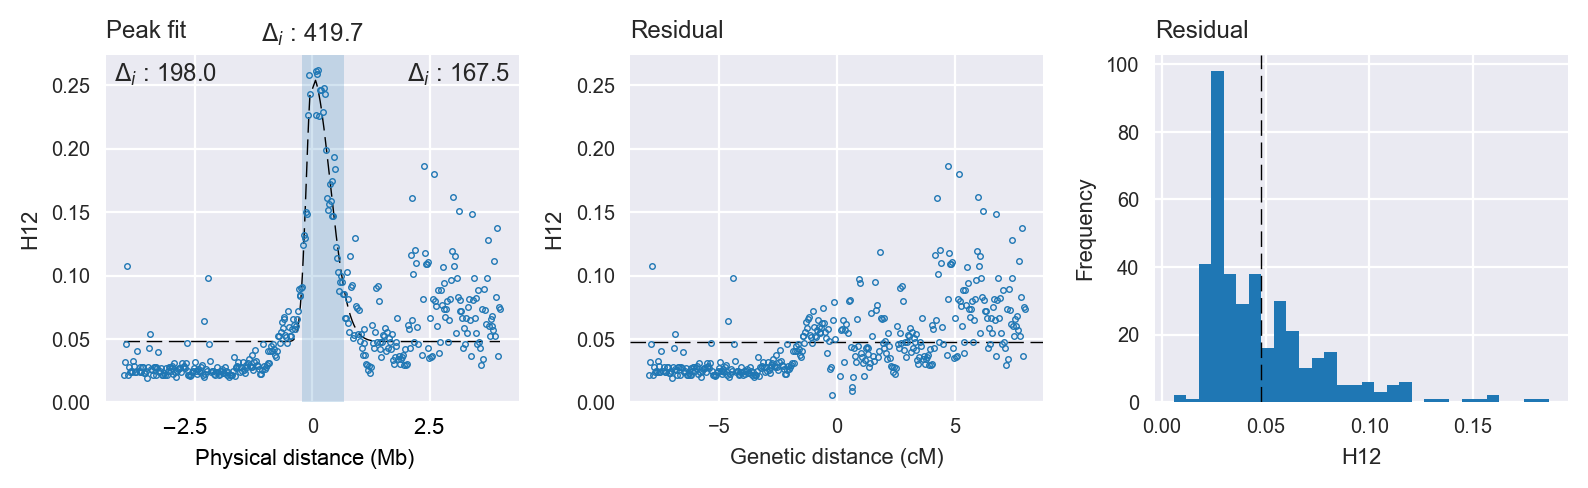
\includegraphics[width=1.1\textwidth,center,trim=0 27 380 0, clip]{artwork/chapter5/peak_fit_h12_cyp9k1_gns.png}
    \end{subfigure}
    \vspace{0cm}
    \begin{subfigure}[t]{0.32\textwidth}
        \centering
        \caption{}
        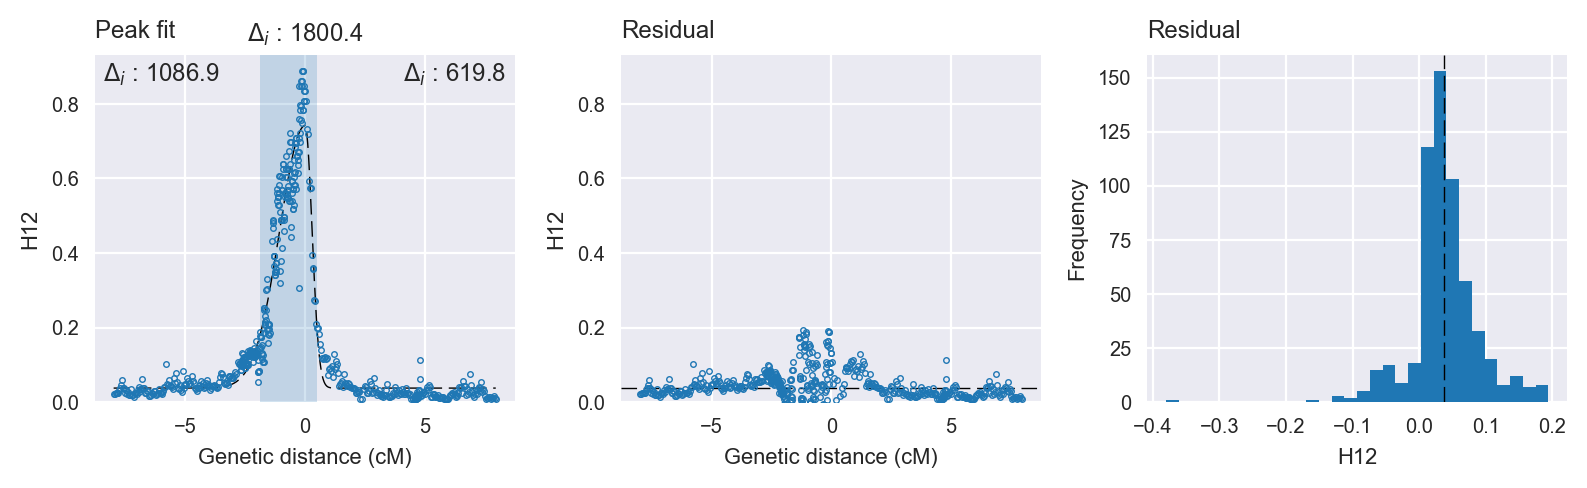
\includegraphics[width=1.1\textwidth,center,trim=0 0 380 0, clip]{artwork/chapter5/peak_fit_h12_vgsc_bfm.png}
    \end{subfigure}
    \hfill
    \begin{subfigure}[t]{0.32\textwidth}
        \centering
        \caption{}
        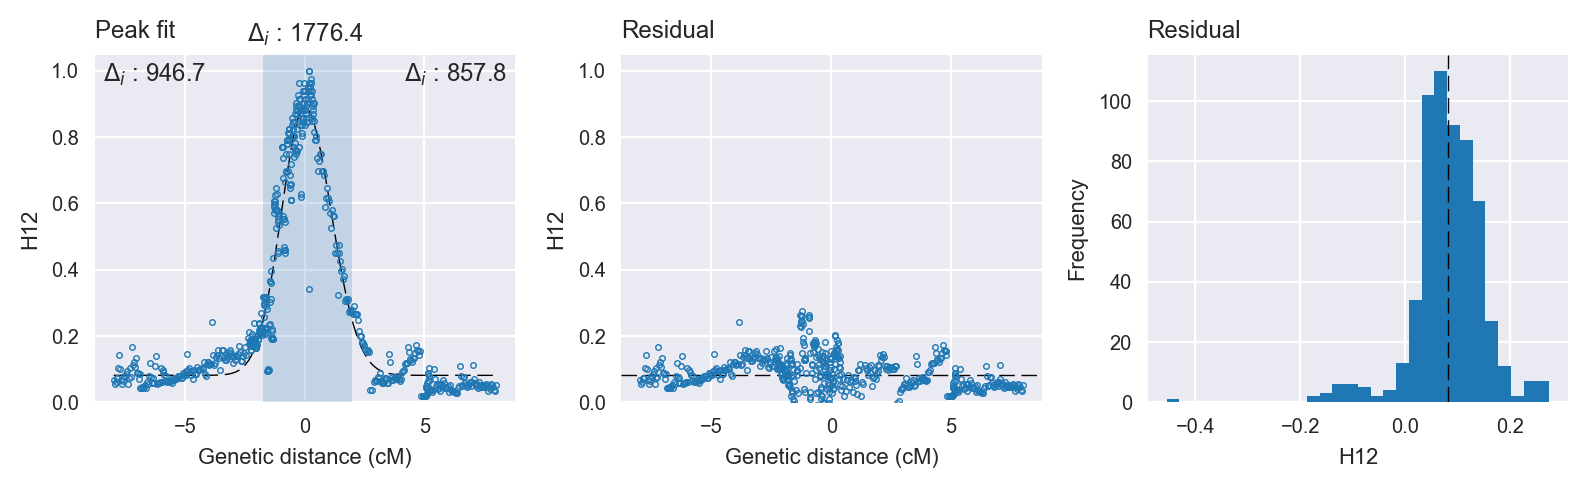
\includegraphics[width=1.1\textwidth,center,trim=0 0 380 0, clip]{artwork/chapter5/peak_fit_h12_vgsc_bfs.png}
    \end{subfigure}
    \begin{subfigure}[t]{0.32\textwidth}
        \centering
        \caption{}
        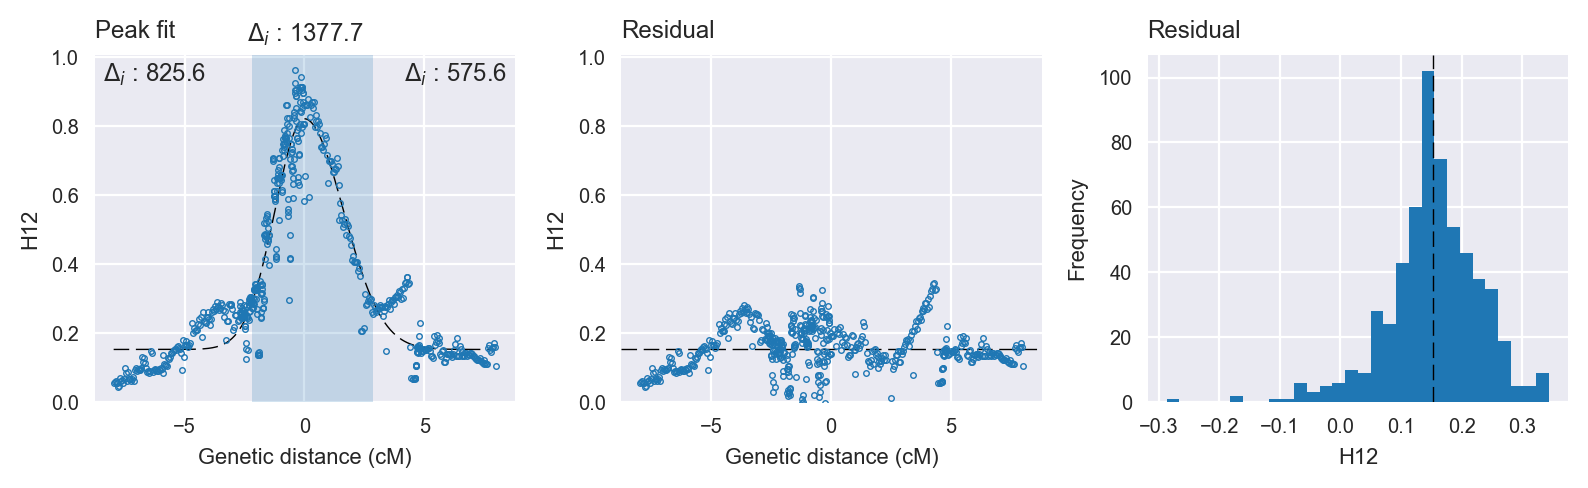
\includegraphics[width=1.1\textwidth,center,trim=0 0 380 0, clip]{artwork/chapter5/peak_fit_h12_vgsc_ugs.png}
    \end{subfigure}
    \caption{Examples of peak models fitted to H12 selection scans at known insecticide resistance loci using least-squares regression. Dashed lines show model fit, markers show data. \textbf{a}, \textit{Cyp6p}, Uganda \agam. \textbf{b}, \textit{Cyp6p}, Burkina Faso \agam. \textbf{c}, \textit{Cyp6p}, Burkina Faso \acol. \textbf{d}, \textit{Gste}, Cameroon \agam. \textbf{e}, \textit{Gste}, Burkina Faso \agam. \textbf{f}, \textit{Gste}, Uganda \agam. \textbf{g}, \textit{Cyp9k1}, Burkina Faso \agam. \textbf{h}, \textit{Cpy9k1}, Burkina Faso \acol. \textit{i}, \textit{Cyp9k1, Guinea \agam}. \textbf{j}, \textit{Vgsc}, Burkina Faso \acol. \textbf{k}, \textit{Vgsc}, Burkina Faso \agam. \textbf{l}, \textit{Vgsc}, Uganda \agam.}
    \label{fig:peak_fits}
\end{figure}


To learn more about the character of signals of selection for insecticide resistance, I studied the selection scan statistics in more detail at the five known insecticide resistance loci listed above.
%
A common feature of selection signals at these loci was a clear peak architecture, with a maximum (peak) value close to the target gene, and values of the selection statistic decaying to background levels both upstream and downstream of the gene.
%
In the H12 selection scans in particular, values on either side of the target gene appeared to decay asymptotically, and it occurred to me to model this decay by fitting exponential functions to each flank of a selection signal via least-squares regression.
%
This exponential peak model provided a good fit to the selection signals at most of the known insecticide resistance loci (e.g., Fig.~\ref{fig:peak_fits}a-g).
%
I also tested several other peak models, and found that a Gaussian peak model provided a better fit in a minority of cases (e.g., Fig.~\ref{fig:peak_fits}h-l).
%
At the \textit{Vgsc} locus the peaks were highly skewed when plotted against physical genome coordinates, but this locus lies on the border of pericentromeric heterochromatin, and this skew could be almost entirely corrected by assuming the heterochromatin recombination rate is @@ lower than euchromatin.
%
I devised a way to quantify the support for these peak models by also fitting a null constant model at the same locus and computing the difference in Akaike Information Criterion ($\Delta_i$) between the peak and null models.
%
In general, when comparing two models, $\Delta_i > 10$ is considered sufficient evidence to reject the model with higher AIC \parencite{Burnham2002}, and at many of the known insecticide resistance loci I observed $\Delta_i > 1000$ indicating strong support for the exponential peak model.
%


A benefit of this approach to modelling and quantifying support for a selection signal, over simply measuring the peak value, is that it integrates evidence not just at the locus under selection but from the flanking regions as well.
%
At a locus under recent positive selection, genetic hitchhiking of neutral variants on either flank of the locus is expected due to linkage disequilibrium, and the probability of linkage is an exponential function of the genetic distance between them~\parencite{MaynardSmith1974}.
%
\textcite{Wiener2011} showed that this theory could be used as a tool for mapping selection signals, by fitting exponential functions to heterozygosity data on either flank of a locus under positive selection via least squares regression.
%
This previous work, and my observations at known insecticide resistance loci, suggested that least squares regression could be used as a general approach to systematic identification and mapping of signals within the selection scans in the Ag1000G populations.
%
In general, previous studies performing genome-wide selection scans such as @@REF have taken a simple approach to peak identification, by setting a constant threshold and then identifying all contiguous genome regions where selection scan values exceed the threshold, taking the position with the maximum value within each such region as the most likely focus of selection.
%
Examining the Ag1000G data, however, it was clear that such an approach would have a number of shortcomings, illustrated in Fig. @@.
%
The essence of these shortcomings is that they do not leverage the information provided by the shape of peaks at true selection signals, both to reduce false positives due to isolated high noise values, and to reduce artificial breaks in peaks caused by low noise values.


Developing this idea further, I devised an algorithm to systematically identify selection signals within each scan, quantify their support, map the most likely focus of selection, and provide some indication of the relative uncertainty surrounding the mapped focus.
%
Briefly, the algorithm uses least squares regression to fit peak and null models to the selection scan values at regular @@ kb intervals throughout the genome.
%
To deal with nearby selection signals where peaks may be partially overlapping, it then proceeds to iteratively identify the peak value with the strongest statistical support, subtract the fitted peak values from the data, and refit peaks in neighbouring regions.
%
I applied this algorithm to the H12, IHS and XPEHH scans in each of the 8 populations.
%
This generated a catalog of @@how many selection signals, which I then ranked by $\Delta_i$.


%%%%%%%%%%%%%%%%%%%%%%%%%%%%%%%%%%%%%%%%%%%%%%%%%%%%%%%%%%%%%%%%%%%%%%%%%%%%%%%
%%%%%%%%%%%%%%%%%%%%%%%%%%%%%%%%%%%%%%%%%%%%%%%%%%%%%%%%%%%%%%%%%%%%%%%%%%%%%%%
\subsection{Validation of signal discovery}\label{subsec:validation}


@@TODO


%%%%%%%%%%%%%%%%%%%%%%%%%%%%%%%%%%%%%%%%%%%%%%%%%%%%%%%%%%%%%%%%%%%%%%%%%%%%%%%
%%%%%%%%%%%%%%%%%%%%%%%%%%%%%%%%%%%%%%%%%%%%%%%%%%%%%%%%%%%%%%%%%%%%%%%%%%%%%%%
%%%%%%%%%%%%%%%%%%%%%%%%%%%%%%%%%%%%%%%%%%%%%%%%%%%%%%%%%%%%%%%%%%%%%%%%%%%%%%%
\section{Conclusions}\label{sec:conclusions}


@@todo


%%%%%%%%%%%%%%%%%%%%%%%%%%%%%%%%%%%%%%%%%%%%%%%%%%%%%%%%%%%%%%%%%%%%%%%%%%%%%%%
%%%%%%%%%%%%%%%%%%%%%%%%%%%%%%%%%%%%%%%%%%%%%%%%%%%%%%%%%%%%%%%%%%%%%%%%%%%%%%%
%%%%%%%%%%%%%%%%%%%%%%%%%%%%%%%%%%%%%%%%%%%%%%%%%%%%%%%%%%%%%%%%%%%%%%%%%%%%%%%
\section{Methods}\label{sec:methods}


@@todo


%%%%%%%%%%%%%%%%%%%%%%%%%%%%%%%%%%%%%%%%%%%%%%%%%%%%%%%%%%%%%%%%%%%%%%%%%%%%%%%
%%%%%%%%%%%%%%%%%%%%%%%%%%%%%%%%%%%%%%%%%%%%%%%%%%%%%%%%%%%%%%%%%%%%%%%%%%%%%%%
%%%%%%%%%%%%%%%%%%%%%%%%%%%%%%%%%%%%%%%%%%%%%%%%%%%%%%%%%%%%%%%%%%%%%%%%%%%%%%%
\section{Acknowledgments}\label{sec:acknowledgments}


@@TODO


\printbibliography


\clearpage
\beginsupplement
%%%%%%%%%%%%%%%%%%%%%%%%%%%%%%%%%%%%%%%%%%%%%%%%%%%%%%%%%%%%%%%%%%%%%%%%%%%%%%%
%%%%%%%%%%%%%%%%%%%%%%%%%%%%%%%%%%%%%%%%%%%%%%%%%%%%%%%%%%%%%%%%%%%%%%%%%%%%%%%
%%%%%%%%%%%%%%%%%%%%%%%%%%%%%%%%%%%%%%%%%%%%%%%%%%%%%%%%%%%%%%%%%%%%%%%%%%%%%%%
\section{Supplemental figures}\label{sec:supplemental-figures}


@@todo


\clearpage
%%%%%%%%%%%%%%%%%%%%%%%%%%%%%%%%%%%%%%%%%%%%%%%%%%%%%%%%%%%%%%%%%%%%%%%%%%%%%%%
%%%%%%%%%%%%%%%%%%%%%%%%%%%%%%%%%%%%%%%%%%%%%%%%%%%%%%%%%%%%%%%%%%%%%%%%%%%%%%%
%%%%%%%%%%%%%%%%%%%%%%%%%%%%%%%%%%%%%%%%%%%%%%%%%%%%%%%%%%%%%%%%%%%%%%%%%%%%%%%
\section{Supplemental tables}\label{sec:supplemental-tables}


@@todo


\end{document}
